\documentclass{article}
\usepackage{amsmath,amsthm,amssymb,amsfonts}
\usepackage{setspace,enumitem}
\usepackage{graphicx}
\usepackage{hyperref}
\usepackage{natbib}
\usepackage{afterpage}
\usepackage{xcolor}
\usepackage{etoolbox}
\usepackage{booktabs}
\usepackage{pdfpages}
\usepackage{multicol}
\usepackage{geometry}
\usepackage{accents}
\usepackage{bbm}
\usepackage{placeins}
\hypersetup{
	colorlinks,
	linkcolor={blue!90!black},
	citecolor={red!90!black},
	urlcolor={blue!90!black}
}

\newtheorem{theorem}{Theorem}
\newtheorem{assumption}{Assumption}
\newtheorem{definition}{Definition}
\newtheorem{lemma}{Lemma}
\setlength{\parindent}{0cm}
\geometry{margin = 1in}

\newcommand{\R}{\mathbb{R}}
\newcommand{\ubar}[1]{\underaccent{\bar}{#1}}
\newcommand{\Int}{\text{Int}}
\newcommand{\xbf}{\mathbf{x}}
\newcommand{\Abf}{\mathbf{A}}
\newcommand{\Bbf}{\mathbf{B}}
\newcommand{\Gbf}{\mathbf{G}}
\newcommand{\bbf}{\mathbf{b}}
\newcommand{\one}{\mathbbm{1}}

\newtoggle{extended}
\settoggle{extended}{false}

\title{ECON 810: Homework 2}
\author{Alex von Hafften }

\begin{document}

\maketitle

\begin{itemize}

\section{Part 1: Data}

\subsection{Earnings gains while employed}

\item I used PSID data with the following filters:

\begin{itemize}

\item Main sample. No SEO oversample.

\item Years 1978-1997 inclusive.

\item Ages 25 to 60 inclusive.

\item Annual hours worked \texttt{e11101} of at least 1800 (= 52 weeks per year minus two weeks for vacation times 36 hours).

\item I use variable \texttt{i11103} (description ``HH Labor Income") as my income variable, $Y_{it}$. I drop observations with zero income and over $e^{12} \approx 163000$.

\item I limit the growth in earnings to doubling or less (i.e. a hundred percent increase in earnings).

\end{itemize} 

\item I compute an annual change in earnings of 7.35\%.

\item See \texttt{part\_1\_1.R} for implementation.

\subsection{Earnings losses while unemployed}

\item I use the iid normal shocks to individuals income over time $\varepsilon \sim_{iid} N(0, 1000)$.

\item See \texttt{part\_1\_2.jl} for the implementation.

\item $\beta_k \approx 0$ for $k \in \{-4,..., -1\}$ and $\beta_k \approx -9000$ for $k \in \{0,..., 5\}$.  This makes sense because the income shock from job loss is permanent.

\item $\gamma_t$ start at around -5000 and increase by 1000 each period. This makes sense because it captures the incremental increase in income.

\begin{tabular}{lr}
\toprule
          & \multicolumn{1}{c}{earnings} \\ 
\cmidrule(lr){2-2} 
          &                          (1) \\ 
\midrule
dm4       &                      113.728 \\ 
          &                     (87.470) \\ 
dm3       &                      122.149 \\ 
          &                     (87.470) \\ 
dm2       &                        7.981 \\ 
          &                     (87.470) \\ 
dm1       &                       80.500 \\ 
          &                     (87.470) \\ 
d0        &                 -8842.457*** \\ 
          &                     (87.470) \\ 
dp1       &                 -8895.236*** \\ 
          &                     (87.470) \\ 
dp2       &                 -8969.840*** \\ 
          &                     (87.470) \\ 
dp3       &                 -8885.697*** \\ 
          &                     (87.470) \\ 
dp4       &                 -8891.502*** \\ 
          &                     (87.470) \\ 
dp5       &                 -8935.596*** \\ 
          &                     (87.470) \\ 
\midrule
\midrule
Estimator &                          OLS \\ 
\midrule
$N$       &                       11,000 \\ 
$R^2$     &                        0.941 \\ 
\bottomrule
\end{tabular}


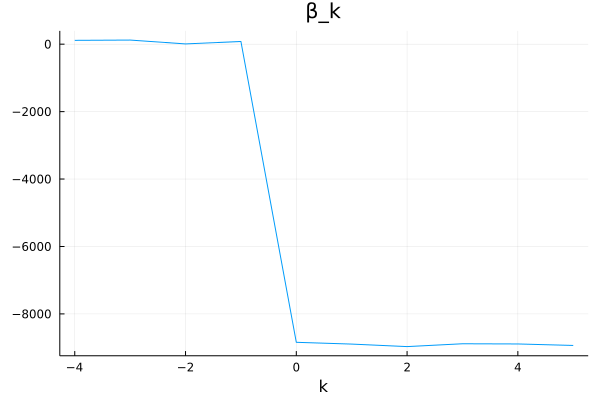
\includegraphics[scale=0.5]{part_1_2_beta}

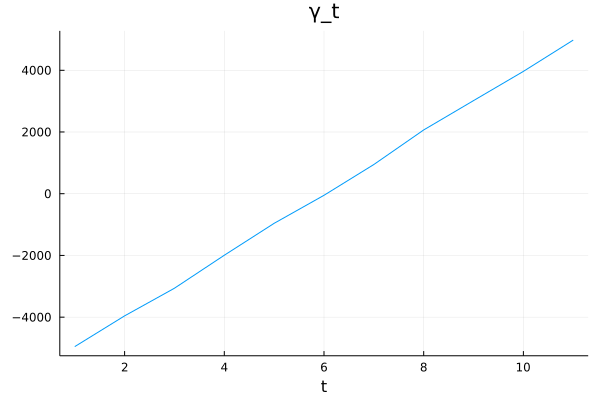
\includegraphics[scale=0.5]{part_1_2_gamma}

\pagebreak

\section{Part 2: Model}

\item See \texttt{part\_2.jl} for implementation.

\end{itemize}
\end{document}

